\documentclass[11pt]{article}

\usepackage[]{ACL2023}

\usepackage{times}
\usepackage{latexsym}

\usepackage[T1]{fontenc}

\usepackage[utf8]{inputenc}

\usepackage{microtype}

\usepackage{inconsolata}

\usepackage{graphicx}

\usepackage{tabularx}

\title{Asking Clarifying Questions for Conversational Search}

\author{
  Ansh Bisht \and
  Jordan Dickson \and
  Jack Harrison \and
  Ruben Lazell \and
  Andrew Taison  \\
  School of Computing, Engineering and the Built Environment, \\
  Edinburgh Napier University \\
  Matric Numbers: 40527530, 40545300, 40537035, 40679914, 40538519
}


\begin{document}
\maketitle
\begin{abstract}
Short abstract.
\end{abstract}


\section{Introduction}
Modern search systems are capable of retrieving large amounts of information, but understanding user intent remains a challenge. Users often submit short and ambiguous queries that make it difficult for retrieval models to determine what information is actually being sought. This gap between what the user means and what the system retrieves can lead to irrelevant or overly broad results. One approach to addressing this problem is through conversational search, where the system interacts with the user by asking clarifying questions before returning results. These questions can help refine the search context, helping to identify intent and improve result relevance. Without clarification, search systems could return unhelpful results leading to user frustration and multiple search requests, potentially at the risk of the user giving up.

This project focuses on building a simple yet functional system that incorporates this idea of clarification. Rather than treating each query as a final standalone input, the system maintains continuous conversation context, considering earlier interactions to inform retrieval and question selection. When a user submits a query, the system first attempts to retrieve a relevant document using an information retrieval method. If the result is assessed to be confident, it is returned directly. If not, the system instead identifies and presents a clarifying question to the user, aiming to narrow down the user's intent. This process can repeat until a high confident match is found.

Developing such a system involves several challenges. The first is determining when to ask a clarifying question and when to present a result. The second is selecting a question that fits naturally into the context of the conversation. Finally, there is the issue of developing the system with limited time and computational resources. Our system addresses these by using a modular architecture with separate components handling retrieval, ranking, and dialogue flow. Clarification decisions are made based on a confidence score from a BM25 retrieval module. If the score is low, a Sentence-BERT (SBERT) model, fine-tuned on multi-turn conversations, is used to select the most suitable clarifying question from a predefined set.

The use of Rasa as the dialogue manager allows us to handle user inputs, manage context history, and direct the flow between modules in a structured way. Each query and response pair is stored as part of a conversation string, which provides context for both the retrieval and question ranking modules. The final system is deliberately kept lightweight to make development manageable whilst supporting clear functionality and reliable testing within the project's constraints.

The remainder of this paper is structured as follows. Section 2 presents related work that informed development. Section 3 explains the system architecture and implementation. Section 4 outlines the evaluation process, whilst Section 5 discusses the system's behaviour and limitations. Section 6 concludes the report and suggests areas for further work.

\section{Related Work}
This project was motivated by recent studies in conversational search, particularly where ambiguity in user queries is addressed by asking clarifying questions. Across the discussed literature, it is commonly noted that users often struggle to express their intent clearly in a single query. Moreover, it is found that even simple follow up questions can help search systems return more relevant results. Whilst our system simplifies many of the models used in previous work, it is inspired by several of their core ideas, adapting them to be lightweight for demonstration purposes and time constraints.

\subsection{Clarification as a Ranking Problem and the Qulac Dataset}
\citet{Aliannejadi2019} examine how clarifying questions can improve conversational search, showing that even a single, well targeted question can significantly improve retrieval performance. To support this, they introduce the Qulac dataset, which extends TREC Web Track topics with crowd sourced question and answer pairs organised by query facets (categories). This dataset has been widely used in related research. In addition to the dataset, they propose a retrieval framework in which both documents and candidate questions are retrieved and ranked based on the user's query and conversational context. Question ranking is performed using a BERT model pre-trained on Wikipedia and fine-tuned on Qulac.

Our system builds on this framework, making use of the Qulac dataset for its high quality question-answer pairs and \citeauthor{Aliannejadi2019}'s multi-turn conversation history extension dataset. Similar to \citeauthor{Aliannejadi2019}, our model treats clarification as a ranking problem, selecting the most relevant question from a fixed set based on the current context, rather than generating questions from scratch.

\subsection{User Behaviour and When to Clarify}
Alongside ranking-based clarification frameworks, other studies have focused on how user behaviour can affect the system and effectiveness. Two notable examples include the CoSearcher system introduced by \citet{Salle2022} and the risk-aware decision model proposed by \citet{Wang2022}. Whilst these works differ in their objectives, both incorporate user simulators and address when and how clarification should take place in conversational search.

\citet{Salle2022} present CoSearcher, a user simulator designed to evaluate search intent refinement in conversational search by modelling different user behaviours. Their main focus was centred around testing how different facet-ranking strategies perform under varying conditions such as low user patience or reduced cooperativeness. The authors experiment with a range of ranking models, including LexVec, and use BERT to classify user responses and determine whether further clarification is necessary. Although Sentence-BERT (SBERT) was initially considered, it was not used as LexVec was found to slightly outperform it. However, the gap between LexVec and SBERT was small and they prioritised computational speed. Our system on the other hand is much smaller in scale and can make use of SBERT's sentence level matching and supervised nature, making implementation more straightforward.

\citet{Wang2022} approach the clarification process as a decision making problem, where the system has to decide whether to ask a question or return a result based on how confident it is. To explore this, they train a reinforcement learning model using a reward function that balances retrieval performance with the length and usefulness of the conversation. Like CoSearcher, they implement a user simulator to represent different behaviours, including tolerance and patience. They use these two parameters to determine how many questions a user will put up with before giving up.

Both studies highlight the importance of choosing not just what to ask, but when to ask it. Whilst our system does not include a user simulator or learning-based decision model, we were influenced by how these papers handle ambiguity and user behaviour. In our case, the decision to clarify or move on is made using a straightforward confidence check from the BM25 module. If the score is high, we assume the summary is a good enough match for the user's intent. If it is low, the system switches to question selection instead. Whilst this is a much simpler method, it follows the same general idea that clarification should depend on context and confidence, rather than being the default.

\subsection{Sentence-Level Semantic Similarity}
Clarifying question selection requires more than just a list of candidates, it also needs a way to evaluate how well each one fits the current query. For that, we use SBERT, introduced by \citet{Reimers2019}, which adapts BERT to produce fixed size sentence embeddings that can be compared directly using cosine similarity. Furthermore, \citeauthor{Reimers2019} show that SBERT is much more efficient than standard BERT, as it allows sentences to be encoded independently. In tasks such as clustering of sentences, they report a reduction in computation time from hours to seconds. Although newer versions such as Sentence-T5 exist and have been found to perform better in some scenarios, SBERT worked well for our needs \cite{Ni2021}. SBERT's ability to compare semantic similarity efficiently, makes it well suited for ranking tasks.

\subsection{Dialogue Management with Rasa}
Rasa is an open-source framework designed for building conversational AI applications, combining natural language understanding (NLU), dialogue management and a modular architecture that supports flexible system design \cite{Rasa2025,XaqtTeam2022}. \citet{Dinesh2021} demonstrate how Rasa can be used in task oriented systems, such as answering student questions related to their academic schedules or syllabuses. Their work shows that even relatively simple applications can benefit from Rasa's modular setup, which allows different components to be added or swapped depending on the task. This made Rasa a good fit for our project, where a way to manage conversational flow was required whilst simultaneously relying on external modules for retrieval and clarification.

\subsection{Question Generation and Generative Approaches}
Whilst our system uses a fixed pool of pre-written clarifying questions, recent work has explored generating them from scratch. \citet{Wang2023} address the challenge of generating clarifying questions in cold-start scenarios, where there is a lack of real-world conversational data. They propose a zero-shot method where question generation is guided using query facets and question templates rather than directly concatenating facets to query input as in previous models. They show that this approach produces more useful and natural questions than previous zero-shot baselines.

\citet{Zhao2024} introduce an intent-aware framework for generating clarifying questions. In their study, verbs are extracted from search results using the user's query based on the idea that these verbs represent the user's intent. These extracted verbs are then combined with templates to produce intent-aware questions, with the goal of helping to avoid vague or unhelpful questions. Their results show that tailoring questions to a user's intent can improve both accuracy and user satisfaction.

Although we do not attempt question generation in our project, these studies helped our understanding of how clarification might be handled in more advanced systems beyond retrieval-based approaches. In particular, they highlight the importance of considering intent and context, and have provided a basis for designing our simpler ranking-based method.

\section{Methodology}



\subsection{System Overview}
The system for the clarification model was constructed through a series of key components:User queries with a question for the system, RASA for application control of the entire system, Best Matching 25 (BM25) model for matching the queries on the Wikipedia Dataset, and SBERT for constructing Sentence Similarity Scores to rank the most appropriate question.

The dependencies and relationships of these components are illustrated Figure 1.

\begin{figure}[htbp]
  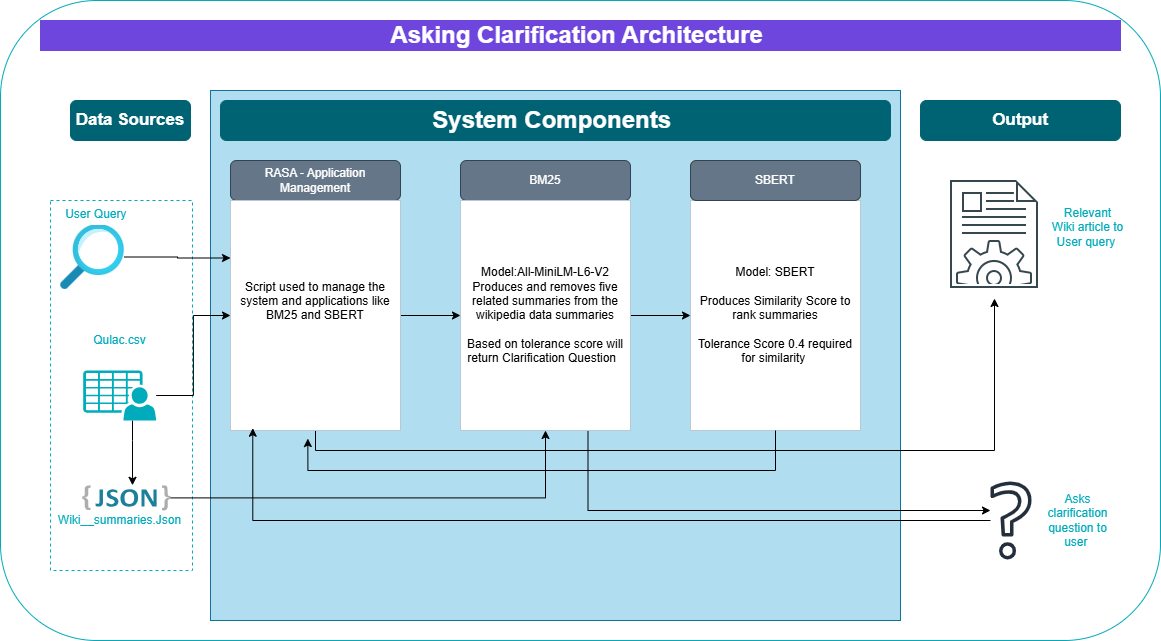
\includegraphics[width=\linewidth]{./img/system_diagram.png}
  \caption{System Diagram for our Clarification project}
  \label{fig:sys_diag}
\end{figure}

\subsection{Qulac Dataset}
The Qulac - short for Questions for Lack of Clarity—is a benchmark dataset created to support research on asking clarifying questions in open-domain, information-seeking conversations and was one of the primary datasets for this system. One of the initial steps was to appropriately shape the data to work with the other elements within our system. The transformations for cleaning this dataset were performed initially in Python using the Pandas library, and the resulting CSV was stored within GitHub.

\subsection{Original Qulac Dataset}
In short the Qulac dataset is a dictionary with query keys and a list of relevant facet descriptions (user intents).

Each query in Qulac is paired with a set of ten candidate clarifying questions, which are designed to resolve potential ambiguity. For example, the query "jaguar" could relate to the animal, the car brand, or even the sports team, and Qulac includes questions such as “Are you referring to the animal or the car brand?” to help systems distinguish between these interpretations. These questions were manually authored and assessed through crowdsourcing to ensure relevance and effectiveness in eliciting more specific user intent. Queries are also accompanied by retrieved web passages from the ClueWeb09 Category B corpus, providing context for question evaluation.

The dataset includes annotations from human judges who rated each candidate question based on its helpfulness, relevance, and clarity. The ratings fall into categories such as excellent, good, fair, or bad, offering a rich signal for training supervised learning models. These annotations allow for the creation of ranking systems that prioritize better clarifying questions over less helpful ones. The inclusion of such human judgments positions Qulac as a valuable dataset for evaluating both neural ranking models and question generation systems in the conversational IR domain.

\subsection{Clean Qulac Schema}
\renewcommand{\arraystretch}{1.2} % increase row height for readability

\begin{table}[ht]
  \centering
  \caption{Transformed Qualac Dataset for BM25 and Wiki Summaries}
  \label{tab:dataset-columns}
  \begin{tabularx}{\columnwidth}{@{} l l X @{}}
    \hline
    \textbf{Column Name}  & \textbf{Type}    & \textbf{Description}                        \\ 
    \hline
    Index                 & String           & Facet index based on word string.            \\ 
    Category Name         & String           & Name of the broader category of the dataset. \\ 
    Facet Description     & String           & Detailed description of the facet.           \\ 
    Col 1                 & String           & Response 1.                                  \\ 
    Col 2                 & String           & Response 2.                                  \\ 
    Col 3                 & String           & Response 3.                                  \\ 
    Col 4                 & String           & Response 4.                                  \\ 
    New Index             & Integer          & Row index counter.                           \\ 
    \hline
  \end{tabularx}
\end{table}

One of the most important features of the Qulac Dataset was the facet descriptions, as they were used to derive the Wikipedia Summaries. A facet is a clarifying intent subtopic to given a query and an facet description is a description of this subtopic. Let us take "Cat" as an example of a facet. In this scenario there are four potential facets for cats; the mammal - felius catus - , the musical  and the shoe brand. The facet description are important as they context to derive from a readable form which of these facets are being used in a certain context. Hence they important for deriving the correct wikipedia summaries. 

\subsection{Wikipedia Summaries}
The Wikipedia summaries were generated using a series of GET responses contained within a Python script on the Wikipedia API. The aim was to generate five summaries per topic based on the facet descriptions \textendash{} relating to the user's query. In short, the facet descriptions were used within a search function as to return the most relevant results within a given context. The reason why five results where generated instead of all possible results was reduce the amount of noise in our dataset. Only the Wikipedia summaries where used to save on performance and time. In a larger and more extensive project, the entire Wikipedia summary should be generated. 

\begin{figure}[htbp]
  \centering
  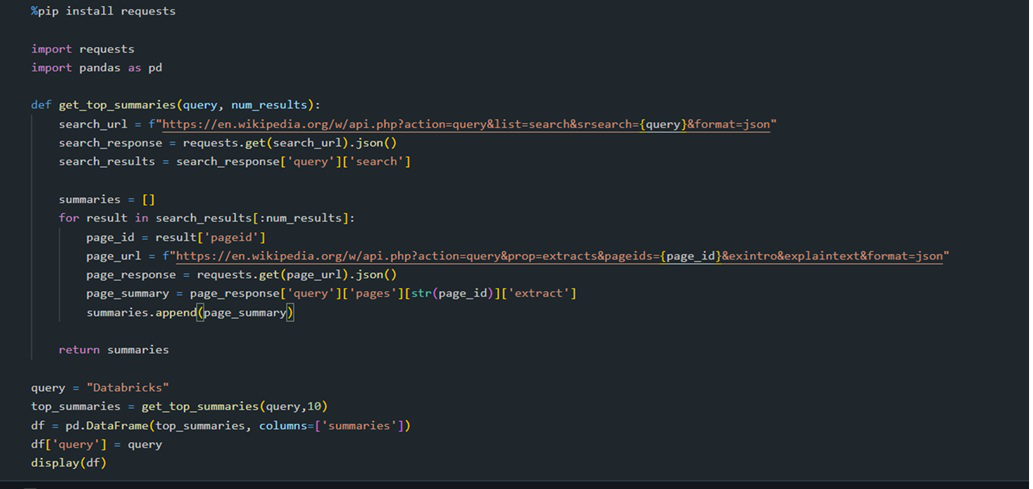
\includegraphics[width=\linewidth]{./img/wiki.png}
  \caption{Wikipedia Summaries Generation}
  \label{fig:wikipedia method}
\end{figure}

In the figure - wikipedia method, a function is used to generate the results of our searches. The method was crafted in this way to ensure that it could retrieve data from the API at ease. If the project was larger in scope, the parameters and a couple of variables could be simply changed to gain the entire wikipedia article. 

Once completed, the Wikipedia Summaries were shaped into the cleaned dataset above. These summaries were required for BM25 later in the project. In a larger project, the Wikipedia API could be used to return the entire articles, but this would come at a cost of time, compute, and complexity.


\subsection{{RASA}}
RASA is the machine learning framework used for building this system. It is used to manage the dialogue by deploying the suitable modules. For this project, RASA deploys BM25 and SBERT, allowing the system to function cohesively. 

\subsection{Best Matching 25 (BM25)}
BM25 was a key ranking function used in the project for informational retrieval within the project. For the project, BM25 ranked the user queries to the relevant Wikipedia summaries giving them a ranking score. This function was imported from Huggingface via a python script. 
 \newline
 \newline
The documents used were the Wikipedia Summaries from the generated CSV. A ranking was also performed using all-MiniLM-L6-v2 from HuggingFace to select the best matching summary.


\subsection{SBERT}
The final step was determining the suitability of the top-ranked question. A specialized version of BERT called SBERT from Huggingface was utilised.

Our SBERT model was fine-tuned on \texttt{sbert\_training\_data.csv}, which contained two features: context and question. Each context is a formatted string combining the initial query and the next element. The model would try to find a similarity between the two strings to rank the relevant results.





\section{Evaluation}
How did we check the system works.
Describe testing process.

\section{Results and Discussion}
Sample outputs.
Summary of system behaviour.
What worked well, what didn't?
Possible improvements.

\section{Conclusion}
start here.

\section*{Limitations}
Required by ACL format, and should be AFTER conclusion.
Discuss honest limitations of the work.

\section*{Ethics Statement}
This project developed a conversational search system for educational demonstrative purposes. All datasets used were publicly available and no personal, sensitive, or specific user data was collected or processed. As the system operates using predefined Wikipedia summaries and clarifying questions, the risk of harm to individuals or groups is minimal. 

\bibliographystyle{acl_natbib}
\bibliography{references}

\appendix

\section{Appendix}
Possibly not needed.

\end{document}
